\documentclass[11pt,a4paper]{article}
\usepackage[margin=24mm,headheight=15pt]{geometry}
\usepackage[T1]{fontenc}
\usepackage{lmodern,microtype,amsmath,amssymb,booktabs,tabularx,array,graphicx,xcolor,fancyhdr,listings,enumitem}
\usepackage[colorlinks=true,linkcolor=black,urlcolor=blue,citecolor=black]{hyperref}
\hypersetup{pdftitle={ML-Based Chemical Process Monitoring Using Gas Sensor Data},pdfauthor={Yug Bhushan}}
\setlength{\parskip}{6pt}\setlength{\parindent}{0pt}
\setlist{nosep,leftmargin=1.5em}\renewcommand{\arraystretch}{1.2}
\pagestyle{fancy}\fancyhf{}\fancyhead[L]{\small ML-Based Chemical Process Monitoring}\fancyhead[R]{\small Yug Bhushan}\fancyfoot[C]{\thepage}
\lstset{language=Python,basicstyle=\ttfamily\scriptsize,breaklines=true,columns=fullflexible,keepspaces=true,showstringspaces=false,frame=single,rulecolor=\color{black!20},numbers=left,numberstyle=\tiny\color{black!50},numbersep=7pt,xleftmargin=10pt,framexleftmargin=5pt}
\newcommand{\sectionpage}[1]{\clearpage\section{#1}}
\begin{document}
\begin{titlepage}\centering\vspace*{22mm}
{\Large\scshape Term Paper\par}\vspace{16mm}
{\huge\bfseries ML-Based Chemical Process Monitoring Using Gas Sensor Data\par}\vspace{10mm}
{\large Principal Component Analysis, Random Forest Classification,\\and Sensor-Drift Evaluation\par}\vspace{24mm}
{\Large Yug Bhushan\par}\vspace{3mm}{\large 2025CH71601\par}\vspace{7mm}
Department of Chemical Engineering\\Indian Institute of Technology Delhi
\vfill{\large Project period: July 2025 -- October 2025\par}\vspace{12mm}
\end{titlepage}

\section*{Abstract}\addcontentsline{toc}{section}{Abstract}
Chemical sensor arrays generate multivariate response patterns that can support gas identification and process monitoring. Their interpretation is complicated by correlated measurements, differences in feature scale, and changes in sensor response over time. This paper develops a machine-learning framework in which principal component analysis (PCA) reduces the dimension of standardized sensor features and a Random Forest classifier assigns observations to six gas classes. The mathematical basis of PCA, tree classification, ensemble aggregation, and multiclass evaluation is presented with a reproducible Python implementation.

The supplied project summary describes more than 13.9 thousand readings from a 16-sensor array and reports 97.8\% accuracy, a 97.6\% F1-score, and 0.99 ROC-AUC on held-out data. These figures are retained as reported project outcomes. The original data, split indices, fitted model, component count, and metric-averaging definitions were not supplied, so the figures are not presented as independently reproduced results. The project description is consistent with the public UCI Gas Sensor Array Drift benchmark, whose feature layout is used to define a compatible reconstruction protocol without asserting that the original files have been verified.

A central distinction is drawn between classification on randomly held-out records and generalization to later measurement batches. PCA can remove redundancy but does not inherently compensate for sensor drift. Temporal evaluation, training-only preprocessing, comparisons with a forest without PCA, and sensor-level permutation analysis are therefore emphasized. Worked numerical examples illustrate PCA variance retention and confusion-matrix metrics. The resulting manuscript provides a methodological foundation and executable analysis workflow while identifying the empirical evidence required to substantiate the reported performance and drift-resistance claims.

\textbf{Keywords:} chemical process monitoring; gas sensor array; principal component analysis; Random Forest; sensor drift; multiclass classification.

\subsection*{Scope of the manuscript}
The project title, period, array size, class count, algorithm family, and reported performance come from the supplied project summary. The temporal split, preprocessing settings, and classifier parameters in this manuscript are proposed reconstruction choices. Numerical examples are explicitly illustrative. Neither a new empirical gas-sensor experiment nor a reproduction of the original performance is claimed.

\clearpage\begingroup\small\tableofcontents\endgroup

\clearpage\section*{Nomenclature}\addcontentsline{toc}{section}{Nomenclature}
\begin{tabularx}{\textwidth}{@{}lXl@{}}\toprule
Symbol & Meaning & Unit or domain\\\midrule
$n$ & Number of measurement records & count\\
$d$ & Number of original features & count\\
$q$ & Number of retained principal components & count\\
$K$ & Number of gas classes & 6\\
$X$ & Matrix of original sensor features & mixed feature units\\
$Z$ & Standardized feature matrix & dimensionless\\
$\mu_j,s_j$ & Training mean and standard deviation of feature $j$ & feature unit\\
$C$ & Sample covariance matrix of standardized features & dimensionless\\
$\lambda_j$ & Eigenvalue of $C$ & dimensionless\\
$v_j$ & Principal-axis loading vector & dimensionless\\
$V_q$ & Matrix of $q$ retained loading vectors & dimensionless\\
$T$ & Matrix of principal-component scores & dimensionless\\
$R_s(t)$ & Resistance response of sensor $s$ & resistance unit\\
$B$ & Number of decision trees & count\\
$p_k$ & Class probability or class proportion & $[0,1]$\\
$G$ & Gini impurity & dimensionless\\
$M_{ij}$ & Confusion count, true class $i$, predicted class $j$ & count\\
TP, FP, FN & True positives, false positives, false negatives & count\\
FPR, TPR & False-positive rate and true-positive rate & $[0,1]$\\
AUC & Area under the receiver operating characteristic curve & $[0,1]$\\\bottomrule
\end{tabularx}

\subsection*{Definitions}
A \emph{measurement record} is one experimental observation represented by an array-derived feature vector. It need not be a single raw sampling instant. A \emph{feature} is a numerical descriptor of a sensor response; a \emph{principal component} is a linear combination of those features. A high-importance component therefore does not directly identify one physical sensor.

\emph{Sensor drift} denotes a change in the relationship between the sensing system's response and the quantity or class of interest. A shifted feature distribution can also arise from changing gas concentrations or class proportions. These mechanisms must be considered when interpreting a decline in classification performance over time.

\sectionpage{Introduction and Engineering Motivation}
\subsection{Multivariate sensing for chemical processes}
Gas monitoring often requires discrimination between several chemical species rather than interpretation of one sensor channel in isolation. An array of partially selective sensors can provide a response pattern whose combined information is more useful than the output of any single sensor. Machine learning maps these patterns to gas identities using labelled examples.

For chemical engineering, such methods connect measurement, statistical analysis, and process understanding. Potential applications include screening process-stream composition, checking the consistency of a measurement system, and identifying unexpected changes that warrant investigation. A gas-identity classifier is one element of a monitoring workflow; it does not directly estimate a continuous concentration, locate a leak, or diagnose every possible process fault.

The distinction between identity and concentration is particularly important. A dataset containing several gas concentrations can be used to classify identity, but a high identity-classification score does not demonstrate accurate concentration measurement. Similarly, a classifier trained on individual gases cannot be assumed to recognize arbitrary mixtures without supporting experiments.

\subsection{Challenges in sensor-array data}
Several feature channels may describe the same underlying response. This creates redundancy and increases the apparent dimension of the problem. Features may also use different scales: an absolute response descriptor and a normalized descriptor should not be allowed to compete solely through numerical magnitude.

A further challenge is temporal stability. A response pattern learned during an early calibration period may shift as the sensing system changes. A model can perform strongly on a random sample from the complete record while performing less well on a later batch. An evaluation design must therefore match the intended use of the model.

\subsection{Objectives and organization}
This paper aims to explain how PCA and Random Forest classification can be combined, develop an evaluation protocol that separates interpolation from future-batch generalization, and interpret the project's reported metrics at the level supported by the supplied evidence. It also provides worked examples, discusses sensor attribution, and documents an executable implementation.

Section 2 defines the data representation. Sections 3 and 4 develop the PCA and forest mathematics. Sections 5 and 6 describe preprocessing, temporal testing, and evaluation. Sections 7 and 8 present illustrative calculations and discuss the reported results. Section 9 addresses limitations and conclusions. The appendices supply the code and execution instructions.

\sectionpage{Dataset Context and Feature Representation}
\subsection{Project description and benchmark compatibility}
The supplied project description states that 13.9K+ multivariate readings were processed from 16 sensors across six gas classes. The UCI Gas Sensor Array Drift dataset contains 13,910 records, six gases, and 16 sensor channels, making it a compatible public benchmark for reconstruction \cite{uci}. This numerical match suggests a likely connection; it does not verify which archive, version, or preprocessing was used in the original project.

The benchmark represents each record with 128 features: eight descriptors for each of 16 sensors. The descriptors summarize resistance response and rising or decaying transients. Records are organized into ten measurement batches. Its class identifiers are listed below. The original dataset contains no missing values according to the repository documentation \cite{uci}.

\begin{table}[h!]\centering
\begin{tabular}{@{}clcl@{}}\toprule
Class & Gas & Class & Gas\\\midrule
1 & Ethanol & 4 & Acetaldehyde\\
2 & Ethylene & 5 & Acetone\\
3 & Ammonia & 6 & Toluene\\\bottomrule
\end{tabular}
\caption{Class labels for the compatible UCI benchmark. The original project label mapping must be checked against its source files.}
\end{table}

\subsection{Proposed input contract}
The implementation accepts a CSV with columns \texttt{batch}, \texttt{class}, and \texttt{x1} through \texttt{x128}. Each row is one record. Class labels must be integers 1--6 and batch identifiers integers 1--10. The feature columns must follow the original sensor grouping: columns 1--8 for sensor 1, columns 9--16 for sensor 2, and so on. This ordering is required for the optional sensor-group permutation analysis.

Batch and class identifiers are metadata, not classifier inputs. Supplying either as a predictive feature would change the task; supplying the true class would directly leak the answer. If concentrations are available, they should be retained as separate metadata for subgroup evaluation rather than silently appended to an identity classifier.

\subsection{Data quality and provenance}
Before fitting, confirm the archive version, units or descriptor definitions, label mapping, batch assignment, and file conversion procedure. Check missing entries, nonfinite values, duplicate records, and unexpectedly constant columns. The code stops on invalid labels, nonfinite features, or duplicated feature vectors so that these cases can be investigated instead of silently changing the experiment.

A negative numerical feature is not automatically invalid: transformed response descriptors may legitimately have either sign. Quality control should use the feature definition rather than an arbitrary positive-value rule. Exact duplicate detection is also distinct from identifying multiple records from the same experimental run. If repeated runs are known, their groups should remain together during splitting.

\sectionpage{Principal Component Analysis: Theory and Derivation}
\subsection{Training-only standardization}
Let $X\in\mathbb R^{n\times d}$ contain the training features. Each column is centered and scaled using training statistics:
\begin{equation}
z_{ij}=\frac{x_{ij}-\mu_j}{s_j},\qquad
\mu_j=\frac{1}{n}\sum_{i=1}^n x_{ij}.
\end{equation}
The implementation uses the population-standard-deviation convention of \texttt{StandardScaler}. The transformed test data use the same $\mu_j$ and $s_j$; no test-set mean is substituted. Standardization matters because PCA maximizes variance, which depends on the measurement scale.

\subsection{Maximum-variance projection}
For centered standardized data $Z$, define
\begin{equation}
C=\frac{Z^TZ}{n-1}.
\end{equation}
The first principal direction is the unit vector $v$ that maximizes the variance of the projected scores:
\begin{equation}
\max_{v^Tv=1} v^TCv.
\end{equation}
Introducing a Lagrange multiplier gives
\begin{equation}
\mathcal L(v,\lambda)=v^TCv-\lambda(v^Tv-1).
\end{equation}
The stationary condition is
\begin{equation}
Cv=\lambda v.
\end{equation}
Thus, the leading eigenvector supplies the first principal direction and its eigenvalue is the associated sample variance. Subsequent orthogonal eigenvectors provide additional components, ordered so that $\lambda_1\geq\lambda_2\geq\cdots\geq0$.

\subsection{Scores, reconstruction, and retained variance}
For $V_q=[v_1,\ldots,v_q]$, component scores and the rank-$q$ reconstruction are
\begin{equation}
T=ZV_q,\qquad \widehat Z=TV_q^T.
\end{equation}
The explained-variance ratio for component $j$ is
\begin{equation}
r_j=\lambda_j\Big/\sum_{\ell=1}^d\lambda_\ell,
\qquad R_q=\sum_{j=1}^q r_j.
\end{equation}
The proposed code uses a 95\% variance target with a full singular-value solver \cite{pca}. This is a reconstruction setting, not an observed component count from the original project. The number retained must be read from the fitted training model.

\clearpage
\subsection{Singular-value interpretation}
A singular value decomposition of the centered standardized matrix is
\begin{equation}
Z=U\Sigma V^T.
\end{equation}
The columns of $V$ are the principal directions, and
\begin{equation}
\lambda_j=\frac{\sigma_j^2}{n-1},
\end{equation}
where $\sigma_j$ is a singular value. This provides a direct numerical route to the projection without explicitly forming a potentially poorly conditioned covariance matrix.

Because each eigenvector can be multiplied by $-1$ without changing its axis, component signs may differ across equivalent implementations. A sign reversal changes score signs but not the represented subspace. Comparisons should therefore account for sign ambiguity rather than treating it as a scientific disagreement.

\subsection{Why PCA may help}
Correlated descriptors can often be represented with fewer coordinates. Reducing dimension can lower storage and prediction cost and provide a compact visualization. In some datasets it may also remove low-variance noise. These are possible benefits, not guaranteed improvements in class discrimination.

PCA is unsupervised: it uses $X$ but not the gas labels. A direction with low overall variance may still separate two classes, while a high-variance direction may mainly reflect concentration or temporal drift. Consequently, a high retained-variance percentage is not equivalent to high predictive accuracy. The variance threshold should be assessed using a training validation design if it is to be tuned.

\subsection{PCA and sensor drift}
A fixed PCA model learns the dominant training subspace. It does not automatically make future observations invariant to sensor aging or other response changes. If drift moves future responses along an important component, the drift is retained. If it introduces a new direction, the projection may discard information in a way that also harms class discrimination.

PCA can participate in a drift-management strategy, but drift compensation requires separate evidence. Relevant tests include comparison with a forest without PCA, accuracy and class recall on later batches, and performance as the temporal separation from calibration increases. The appropriate conclusion is determined by those tests rather than by the presence of a PCA step alone.

\subsection{Optional monitoring quantities}
PCA also permits reconstruction-based diagnostics. For a standardized observation $z$, a squared prediction error is
\begin{equation}
Q=\|z-zV_qV_q^T\|_2^2.
\end{equation}
A score-space statistic can be formed as $T^2=t\Lambda_q^{-1}t^T$ when retained eigenvalues are positive. Large values may flag departures from the training representation. These diagnostics require thresholds calibrated on appropriate reference data and are not implemented as alarms in the appendix. A high value is evidence of an unusual response, not proof of a particular process fault.

\sectionpage{Random Forest Classification}
\subsection{Decision-tree splits}
A classification tree partitions feature space using rules such as $t_j\leq a$, where $t_j$ is a component score. At a node with class proportions $p_1,\ldots,p_K$, the Gini impurity is
\begin{equation}
G=1-\sum_{k=1}^Kp_k^2.
\end{equation}
A pure node has $G=0$. For a proposed split into left and right child nodes, the impurity decrease is
\begin{equation}
\Delta G=G_{\mathrm{parent}}-\frac{n_L}{n}G_L-\frac{n_R}{n}G_R.
\end{equation}
With class weights, the corresponding weighted sample masses replace the raw counts. A tree chooses a candidate split that improves its criterion, then repeats the procedure subject to stopping rules.

\subsection{Ensemble construction and probabilities}
A Random Forest fits many trees using bootstrap samples and random subsets of candidate features. This introduces diversity and reduces dependence on one fitted tree \cite{rf}. For the scikit-learn classifier used here, the forest probability is the average of its tree probabilities:
\begin{equation}
\widehat p_k(x)=\frac{1}{B}\sum_{b=1}^B\widehat p_{k,b}(x),\qquad
\widehat y=\arg\max_k\widehat p_k(x).
\end{equation}
These scores support multiclass ROC analysis, but they are not automatically calibrated probabilities under future distribution shifts.

\subsection{Proposed parameter choices}
\begin{tabularx}{\textwidth}{@{}lX@{}}\toprule
Setting & Reconstruction choice and role\\\midrule
Number of trees & 300; controls ensemble size and computational cost.\\
Minimum leaf size & 2; avoids leaves supported by only one observation.\\
Candidate features & Square root of available input dimension at each split.\\
Class weights & Balanced; inversely related to training class frequencies.\\
Random seed & 42; supports reproducibility of this implementation.\\\bottomrule
\end{tabularx}

These values are explicit implementation choices, not recovered historical settings. Class weighting does not eliminate the need to inspect minority-class errors. Moreover, a forest without PCA uses a different effective candidate-feature count under the square-root rule because its input dimension differs. The comparison is an operational ablation of two pipelines, not a perfectly isolated intervention on projection alone.

\subsection{Feature space and decision boundaries}
A tree built on principal components divides the rotated score space. Those splits correspond to combinations of original sensor features, not necessarily simple thresholds on individual sensor channels. A forest can model nonlinear class boundaries through many piecewise partitions even though PCA itself is linear.

\sectionpage{Computational Workflow and Drift-Aware Validation}
\subsection{Leakage-resistant processing}
The workflow is: validate records, define the split, fit training standardization, fit training PCA, train the forest, and evaluate untouched test rows. A scikit-learn \texttt{Pipeline} keeps the learned transformations attached to their classifier. Applying PCA to the complete dataset before splitting would expose the training procedure to the future feature distribution, even though PCA does not use labels.

Missing-value handling, feature selection, variance thresholds, and classifier tuning must follow the same boundary. If tuning is required, it belongs in an inner validation scheme formed from the training period. The final test data should not be reused to select the preferred parameters or sensors.

\subsection{Two evaluation questions}
\begin{table}[h!]\centering\small
\begin{tabularx}{\textwidth}{@{}lXX@{}}\toprule
Protocol & Proposed split & Interpretation\\\midrule
Random holdout & Stratified 80\% training and 20\% test records across the supplied dataset. & Performance on unseen records from a mixture of observed batches.\\
Temporal holdout & Train on batches 1--6; test on batches 7--10. & Generalization from earlier to later measurement batches.\\\bottomrule
\end{tabularx}
\caption{Proposed reconstruction protocols. Neither split is asserted to be the original project's split.}
\end{table}
The default code implements the temporal protocol. Its optional random protocol is a separate diagnostic run. Random splitting is unsuitable as the sole evidence for future-batch drift resistance. Where multiple records belong to one exposure or run, a group-aware split is also needed; the CSV contract does not contain those groups, so that extension is not implemented.

\subsection{Baselines and ablation}
Three models are compared on identical test rows: PCA plus Random Forest, a Random Forest without PCA, and a majority-class baseline fitted from training labels. The raw-feature forest tests whether projection helps the full classification pipeline. The majority baseline establishes the performance available from the most common training class alone.

Transformations are refitted separately for each protocol. Temporal and random scores answer different questions and belong in separate result tables.

\subsection{Per-batch reporting and retraining}
A single pooled score can hide a large decline in a small or distant batch. The implementation therefore reports metrics for each test batch as well as for their pooled observations. Batch-wise class support must accompany those scores because absent classes make some metrics undefined or change their interpretation.

An expanding-batch extension would predict each new batch using only earlier batches, then update. This differs from fixed calibration, is not implemented here, and requires separate reporting.

\sectionpage{Performance Metrics and Sensor Attribution}
\subsection{Confusion matrix, accuracy, and F1}
Let $M_{ij}$ count records with actual class $i$ and predicted class $j$. Accuracy is
\begin{equation}
\mathrm{Accuracy}=\frac{\sum_kM_{kk}}{\sum_{i,j}M_{ij}}.
\end{equation}
For class $k$, a one-versus-rest interpretation gives
\begin{equation}
\mathrm{Precision}_k=\frac{TP_k}{TP_k+FP_k},\quad
\mathrm{Recall}_k=\frac{TP_k}{TP_k+FN_k},\quad
F1_k=\frac{2TP_k}{2TP_k+FP_k+FN_k}.
\end{equation}
Macro F1 averages class F1 scores equally. Weighted F1 weights them by class support. Micro F1 aggregates counts before computing F1; for ordinary single-label multiclass classification with all classes included, it equals accuracy. Therefore, 97.8\% accuracy and 97.6\% F1 do not identify the averaging convention, and cannot be assumed to be an exact micro-F1 pair on the same predictions.

The code reports both six-class macro F1 and weighted F1. A class with zero support and no predictions receives F1 zero under the explicit \texttt{zero\_division=0} convention. This choice makes per-batch six-class macro F1 conservative but can penalize a batch for classes absent from it. Balanced accuracy averages recall over the classes actually present in that evaluation subset. These definitions should remain visible when interpreting batch comparisons.

\subsection{Multiclass ROC-AUC}
For one class against the rest,
\begin{equation}
\mathrm{TPR}=TP/(TP+FN),\qquad \mathrm{FPR}=FP/(FP+TN).
\end{equation}
Varying a probability threshold produces a ROC curve. AUC summarizes ranking across thresholds; it is different from accuracy at the largest-probability decision rule. The proposed metric is macro one-versus-rest AUC, using probability columns in the same order as the class labels \cite{auc}.

If an evaluation subset lacks positive or negative examples for a class, that binary AUC is undefined. The code leaves the full six-class macro AUC blank unless all six one-versus-rest values are defined. It does not silently average a different set of classes. The reported project AUC of 0.99 remains unspecified as to averaging and multiclass strategy until the original calculation is available.

\subsection{From component importance to sensor importance}
Forest impurity importance after PCA describes the principal components. PCA loadings describe how raw variables contribute to those components. Neither directly supplies a causal ranking of physical sensors. A useful alternative is to permute a raw sensor's eight columns together, pass the perturbed inputs through the complete fitted pipeline, and measure the decrease in held-out balanced accuracy \cite{permutation}.

The optional code repeats this group permutation three times per sensor. It estimates reliance of this fitted pipeline on the grouped information. Correlated sensors can substitute for one another, and a low score does not prove a sensor is dispensable. Selecting a reduced sensor set requires a separate training-validation exercise and an untouched final test.

\addtocontents{toc}{\protect\newpage}
\sectionpage{Illustrative Numerical Analysis}
\subsection{Two-feature PCA calculation}
Consider two standardized features with the hypothetical covariance matrix
\begin{equation}
C=\begin{bmatrix}1&0.8\\0.8&1\end{bmatrix}.
\end{equation}
The characteristic equation is
\begin{equation}
\det(C-\lambda I)=(1-\lambda)^2-0.8^2=0,
\end{equation}
which gives $\lambda_1=1.8$ and $\lambda_2=0.2$. Corresponding unit eigenvectors are
\begin{equation}
v_1=\frac{1}{\sqrt2}\begin{bmatrix}1\\1\end{bmatrix},\qquad
v_2=\frac{1}{\sqrt2}\begin{bmatrix}-1\\1\end{bmatrix}.
\end{equation}
The first direction retains 90\% of total variance. A 90\%-or-greater mathematical retention rule permits one component; a 95\% target requires both components. Numerical libraries may apply a strict threshold convention at exact equality, so the selected count should always be recorded from the fitted object. For $z=(1,2)$, the scores along these selected axes are $3/\sqrt2$ and $1/\sqrt2$.

\begin{figure}[h!]\centering
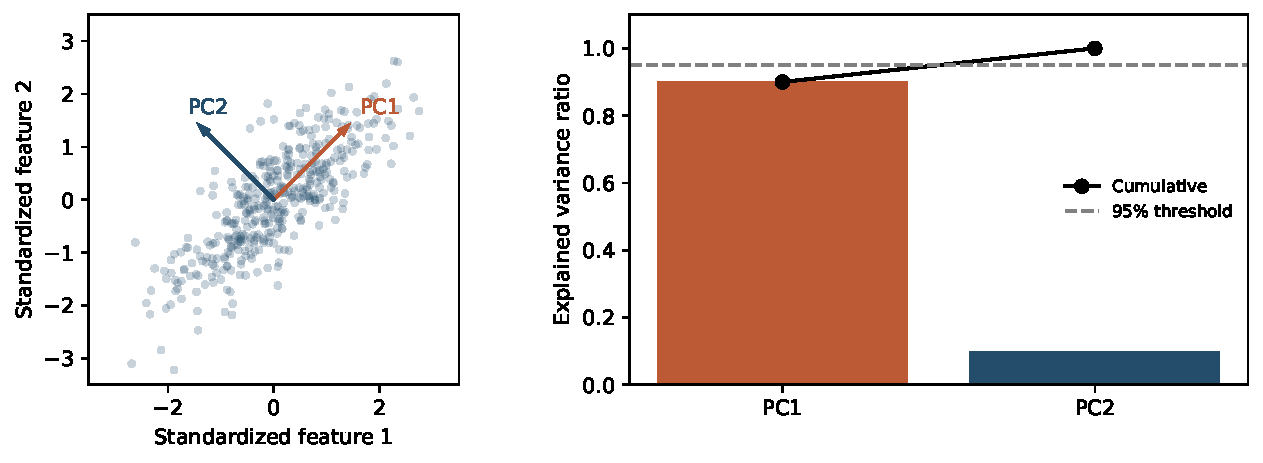
\includegraphics[width=\textwidth]{pca_example.pdf}
\caption{Illustrative correlated features and theoretical variance ratios. The point cloud is generated for explanation and is not a plot of project observations.}
\end{figure}

\subsection{What variance retention does not prove}
If the two gas classes differ primarily along $v_2$, retaining only $v_1$ can remove useful discrimination even though it preserves most variance. If a drift shift lies along $v_1$, retaining the leading component preserves that shift. These examples explain why dimensionality reduction and drift compensation require separate validation.

\clearpage
\subsection{Illustrative six-class confusion matrix}
The following constructed matrix has 20 records per class and is included only to demonstrate metric calculation. It is not the confusion matrix behind the reported 97.8\% accuracy.
\begin{table}[h!]\centering
\begin{tabular}{@{}crrrrrr@{}}\toprule
Actual / predicted & 1&2&3&4&5&6\\\midrule
1&19&1&0&0&0&0\\
2&0&18&0&0&2&0\\
3&0&0&19&1&0&0\\
4&0&0&0&20&0&0\\
5&1&0&0&0&18&1\\
6&0&0&1&0&0&19\\\bottomrule
\end{tabular}
\caption{Illustrative class-count matrix, with rows as actual labels.}
\end{table}
The diagonal totals 113 correct predictions from 120 observations:
\begin{equation}
\mathrm{Accuracy}=113/120=94.1667\%.
\end{equation}
For class 2, $TP_2=18$, $FP_2=1$, and $FN_2=2$. Therefore,
\begin{equation}
\mathrm{Precision}_2=18/19=0.9474,\qquad
\mathrm{Recall}_2=18/20=0.9,
\end{equation}
\begin{equation}
F1_2=36/(36+1+2)=0.9231.
\end{equation}
Averaging the six class F1 scores yields approximately 0.94145. Equal class supports make macro and support-weighted F1 equal in this particular example. In an imbalanced dataset they generally differ.

\subsection{Why AUC cannot be recovered from this matrix}
A confusion matrix records only the final predicted labels. It does not retain the probability ranking across thresholds. Several classifiers can have exactly this matrix while producing different ROC curves and AUC values. No AUC is assigned to the illustrative matrix because probability scores have not been specified.

\subsection{Interpreting an error rate}
A reported 97.8\% accuracy corresponds to a 2.2\% error rate on the stated evaluation set, subject to rounding. The exact error count cannot be calculated without its size. Multiplying 2.2\% by all 13.9K+ project records would incorrectly assume that every record belonged to the held-out test set. Moreover, an average error rate alone does not reveal which gases are confused or whether performance deteriorates in later batches.

\sectionpage{Reported Project Results and Discussion}
\subsection{Performance figures supplied by the project summary}
\begin{table}[h!]\centering\small
\begin{tabularx}{\textwidth}{@{}lXX@{}}\toprule
Item & Reported value & Evidence needed for reproduction\\\midrule
Dataset size & 13.9K+ readings & Original files and preprocessing record.\\
Array and labels & 16 sensors, six gas classes & Feature-to-sensor and label mappings.\\
Method & PCA followed by Random Forest & Training transformations, retained components, classifier settings.\\
Accuracy & 97.8\% on held-out data & Test indices, labels, and predictions.\\
F1-score & 97.6\% & Averaging rule and per-class scores.\\
ROC-AUC & 0.99 & Probability scores, class order, multiclass strategy and averaging.\\
Key sensor features & Identified, according to summary & Importance method, scores, and validation.\\\bottomrule
\end{tabularx}
\caption{Reported outcomes, not independently reproduced results.}
\end{table}

The summary supports describing a PCA--Random Forest project and quoting its reported metrics with attribution. It does not support inventing a retained dimension, naming a best sensor, assigning a confusion matrix, or claiming that a particular temporal experiment produced those values.

\subsection{Classification quality and temporal robustness}
The reported accuracy and F1 suggest strong held-out classification under the original evaluation conditions. Their practical meaning depends on whether test records share batch conditions with training records. If observations were split randomly across all batches, the metrics measure a different generalization task from training early and predicting late.

To support a claim of drift handling, the original experiment should identify its temporal ordering and compare later-batch performance with a meaningful reference. A PCA--forest pipeline should also be compared with the same family's raw-feature pipeline on identical later records. A good random holdout score by itself cannot establish that temporal response changes have been resolved.

\subsection{Sensor interpretation and process relevance}
The project summary mentions isolating key sensor features, but no importance ranking was supplied. A component-based ranking must be distinguished from a raw-feature ranking, and both from a physical sensor ranking. The optional group-permutation calculation provides a reproducible diagnostic once the actual feature ordering is checked.

High classification scores on a laboratory benchmark are useful evidence for algorithm development. Industrial transfer would additionally depend on the gases, concentration range, ambient conditions, acquisition hardware, and mixture patterns encountered in the target application. Those operating conditions are outside the evidence supplied for this paper.

\sectionpage{Limitations, Future Work, and Conclusions}
\subsection{Limitations of the present evidence and model}
The original training data, split indices, model artifacts, and predictions were not provided. Consequently, this manuscript documents reported performance rather than validating the exact historical experiment. The public benchmark provides a compatible data structure, but it cannot identify the original workflow by itself.

PCA may discard low-variance class information, and a forest can learn batch-specific patterns that do not persist. Changes in concentration distribution or class proportions can also affect performance independently of physical sensor drift. These effects should be separated where metadata permit rather than assigning every temporal change to sensor aging.

Uncertainty also matters. A single seed supplies a reproducible partition but not a confidence interval. Independent-row resampling can overstate certainty when records share experimental runs. Group-level or batch-aware uncertainty estimates are preferable when supported by the acquisition design. A ten-batch record provides only limited independent temporal units, which should constrain the strength of generalization claims.

\subsection{Future experimental and computational work}
A useful next study would report fixed-calibration and expanding-batch results side by side, preserving the original batch structure. It would test a modest set of PCA variance thresholds using only early validation batches and compare against a raw-feature forest. Class-wise recall and later-batch confusion patterns would help identify whether errors concentrate on chemically or statistically similar response patterns.

Sensor selection should be treated as a model-development problem rather than inferred from one importance chart. Grouped permutation can motivate candidate subsets, but a refitted reduced-array model must be assessed on a separate final test. Concentration subgroups, mixtures, and environmental changes are further evaluation axes if suitable observations exist.

A deployment study would also distinguish classification confidence from out-of-distribution detection. An unfamiliar sample can receive a high maximum forest probability. Any rejection rule or monitoring threshold therefore requires its own validation and a clear response procedure; it cannot be justified from overall accuracy alone.

\subsection{Conclusions}
PCA and Random Forest provide a practical framework for learning gas identities from multivariate sensor patterns. PCA produces an orthogonal representation of training variance, while the forest learns nonlinear decision regions in that representation. A reliable analysis preserves the training/test boundary through every preprocessing step and reports metrics whose class averaging and probability conventions are explicit.

The supplied project summary reports 97.8\% accuracy, 97.6\% F1-score, and 0.99 ROC-AUC for a six-class, 16-sensor project. Those figures are retained as reported outcomes. The central methodological conclusion is that dimensionality reduction, classification quality, and drift resistance are separate properties. Temporal holdouts, no-PCA comparisons, per-batch errors, and carefully defined sensor attribution are required to connect them. The Python appendix provides a transparent reconstruction protocol for performing those checks when the original observations are available.

\appendix\clearpage\section{Python Implementation}
The code below implements the proposed protocol. It is not the original project script and does not reproduce the reported scores without the original observations and experiment definition. Default temporal testing trains on batches 1--6 and evaluates batches 7--10. Optional random splitting answers a separate diagnostic question. The program writes actual metrics only after receiving a validated input CSV.
\lstinputlisting{gas_sensor_analysis.py}

\clearpage\section{Execution and Reproducibility Notes}
\subsection{Files, environment, and input}
The source project contains \texttt{main.tex}, \texttt{pca\_example.pdf}, and \texttt{gas\_sensor\_analysis.py}. The LaTeX file includes the Python script as a listing, so the script does not need to run during PDF compilation. Upload the complete source archive to Overleaf and use pdfLaTeX, or compile locally until the table of contents is stable.

For the analysis, install Python with NumPy, pandas, Matplotlib, and scikit-learn, and record their versions. Prepare a CSV with \texttt{batch}, \texttt{class}, and exactly named feature columns \texttt{x1} through \texttt{x128}. Preserve the benchmark feature ordering when converting its source files. The CSV's class mapping must agree with Table 1 if gas names are to be assigned to numeric labels.

The default temporal experiment is run with:
\begin{lstlisting}[language={}]
python gas_sensor_analysis.py sensor_data.csv --out temporal_results
\end{lstlisting}
A separate random-holdout diagnostic can be run with:
\begin{lstlisting}[language={}]
python gas_sensor_analysis.py sensor_data.csv --protocol random --out random_results
\end{lstlisting}
To add the optional physical-sensor-group diagnostic, append \texttt{--importance}. The default forest has 300 trees. The \texttt{--trees} argument permits a different declared ensemble size; changing it changes the experiment. Synthetic data used to check execution are not a substitute for project observations.

\subsection{Outputs and interpretation}
\begin{tabularx}{\textwidth}{@{}lX@{}}\toprule
File & Purpose\\\midrule
\texttt{metrics.csv} & Pooled and per-batch metrics for all three models.\\
\texttt{split\_indices.csv} & Zero-based source-row indices of training and test records.\\
\texttt{predictions.csv} & PCA--forest labels and ordered class probabilities.\\
\texttt{pca\_variance.csv} & Retained components, variance ratios, cumulative retention.\\
\texttt{pca\_loadings.csv} & Principal axes in standardized raw-feature coordinates.\\
\texttt{classification\_report.csv} & Per-class precision, recall, F1, and support.\\
\texttt{confusion\_matrix.csv/.png} & Class-count matrix and visualization.\\
\texttt{sensor\_group\_importance.csv} & Optional grouped permutation score drops.\\\bottomrule
\end{tabularx}

A blank six-class macro AUC means at least one binary one-versus-rest AUC is undefined. It is not a zero score. Per-batch F1 and balanced accuracy follow the conventions described in Section 6. Row indices refer to the input CSV's original order after its header; retain the input unchanged if those indices are to remain traceable.

\clearpage\begin{thebibliography}{9}\addcontentsline{toc}{section}{References}
\bibitem{project} User-supplied project summary. \emph{ML-Based Chemical Process Monitoring Using Gas Sensor Data}. Project period July--October 2025. Source of the reported scope and performance figures.
\bibitem{uci} A. Vergara. \emph{Gas Sensor Array Drift Dataset}. UCI Machine Learning Repository, 2012. \url{https://archive.ics.uci.edu/dataset/224/gas+sensor+array+drift+dataset}. Accessed November 5, 2026. Used as a compatible benchmark reference, not a verified copy of the project's original files.
\bibitem{pca} Scikit-learn Developers. \emph{PCA}. Official documentation. \url{https://scikit-learn.org/stable/modules/generated/sklearn.decomposition.PCA.html}. Accessed November 5, 2026.
\bibitem{rf} Scikit-learn Developers. \emph{RandomForestClassifier}. Official documentation. \url{https://scikit-learn.org/stable/modules/generated/sklearn.ensemble.RandomForestClassifier.html}. Accessed November 5, 2026.
\bibitem{auc} Scikit-learn Developers. \emph{roc\_auc\_score}. Official documentation. \url{https://scikit-learn.org/stable/modules/generated/sklearn.metrics.roc_auc_score.html}. Accessed November 5, 2026.
\bibitem{permutation} Scikit-learn Developers. \emph{Permutation feature importance}. Official documentation. \url{https://scikit-learn.org/stable/modules/permutation_importance.html}. Accessed November 5, 2026.
\bibitem{metrics} Scikit-learn Developers. \emph{Metrics and scoring: quantifying the quality of predictions}. Official documentation. \url{https://scikit-learn.org/stable/modules/model_evaluation.html}. Accessed November 5, 2026.
\end{thebibliography}
\end{document}
